\documentclass{article}
\usepackage{fleqn}
\usepackage{epsf}

\usepackage{aima2e-slides}

\begin{document}

\begin{huge}
\titleslide{Học tăng cường (Reinforcement learning)}{Chương 21, Phần 1--4}

\sf

%%%%%%%%%%%% Slide 2 %%%%%%%%%%%%%%%%%%%%%%%%%%%%%%%%%%%%%%%%%%%%%%%%%%%
\heading{Phác thảo}

\blob Các ví dụ

\blob Học một hàm giá trị cho một chính sách cố định

\note{-- học qua khác biệt thời gian (temporal difference learning)}

\blob Học Q (Q-learning)

\blob Xấp xỉ hàm (Function approximation)

\blob Khám phá (Exploration)

%%%%%%%%%%%% Slide 3 %%%%%%%%%%%%%%%%%%%%%%%%%%%%%%%%%%%%%%%%%%%%%%%%%%%
\heading{Học tăng cường}

\blob Tác tử nằm trong môi trường MDP hoặc POMDP

\blob Phản hồi duy nhất cho việc học là nhận thức + phần thưởng (percept + reward)

\blob Tác tử phải học một chính sách dưới dạng nào đó:

\note{-- mô hình chuyển tiếp $T(s, a, s')$ cộng với hàm giá trị $U(s)$}

\note{-- $Q(a,s)$ = tiện ích kỳ vọng nếu chúng ta thực hiện $a$ trong $s$ và sau đó hành động tối ưu}

\note{-- chính sách $\pi(s)$}

%%%%%%%%%%%% Slide 4 %%%%%%%%%%%%%%%%%%%%%%%%%%%%%%%%%%%%%%%%%%%%%%%%%%%
\heading{Ví dụ: Thế giới 4x3}

\vspace*{0.2in}
$(1,1) \stackrel{-.04}{\longrightarrow} (1,2) \stackrel{-.04}{\longrightarrow} (1,3) \stackrel{-.04}{\longrightarrow} (1,2) \stackrel{-.04}{\longrightarrow} (1,3) \stackrel{-.04}{\longrightarrow} \dots (4,3) +1$

\vspace*{0.2in}
$(1,1) \stackrel{-.04}{\longrightarrow} (1,2) \stackrel{-.04}{\longrightarrow} (1,3) \stackrel{-.04}{\longrightarrow} (2,3) \stackrel{-.04}{\longrightarrow} (3,3) \stackrel{-.04}{\longrightarrow} \dots (4,3) +1$

\vspace*{0.2in}
$(1,1) \stackrel{-.04}{\longrightarrow} (2,1) \stackrel{-.04}{\longrightarrow} (3,1) \stackrel{-.04}{\longrightarrow} (3,2) \stackrel{-.04}{\longrightarrow} (4,2) -1$

%%%%%%%%%%%% Slide 5 %%%%%%%%%%%%%%%%%%%%%%%%%%%%%%%%%%%%%%%%%%%%%%%%%%%
\heading{Ví dụ: Backgammon}

\blob Phần thưởng cho thắng/thua chỉ có ở trạng thái kết thúc, còn lại là 0

\blob TDGammon học $\hat{U}(s)$, biểu diễn dưới dạng mạng nơ-ron 3 lớp

\blob Kết hợp với tìm kiếm độ sâu 2 hoặc 3, trở thành một trong ba người chơi giỏi nhất thế giới

%%%%%%%%%%%% Slide 6 %%%%%%%%%%%%%%%%%%%%%%%%%%%%%%%%%%%%%%%%%%%%%%%%%%%
\heading{Ví dụ: Học ở động vật}

\blob RL đã được nghiên cứu thực nghiệm hơn 60 năm trong tâm lý học

\blob Phần thưởng: thức ăn, đau đớn, cơn đói, dược phẩm giải trí, v.v.

\blob Ví dụ: ong học kế hoạch tìm kiếm thức ăn gần tối ưu trong cánh đồng hoa nhân tạo với nguồn mật được kiểm soát

\blob Ong có một kết nối nơ-ron trực tiếp từ bộ phận đo lượng mật nạp vào tới vùng lập kế hoạch vận động

%%%%%%%%%%%% Slide 7 %%%%%%%%%%%%%%%%%%%%%%%%%%%%%%%%%%%%%%%%%%%%%%%%%%%
\heading{Ví dụ: Trực thăng tự trị}

\blob Phần thưởng = -- bình phương độ lệch so với trạng thái mong muốn

\vspace*{0.2in}
\centerline{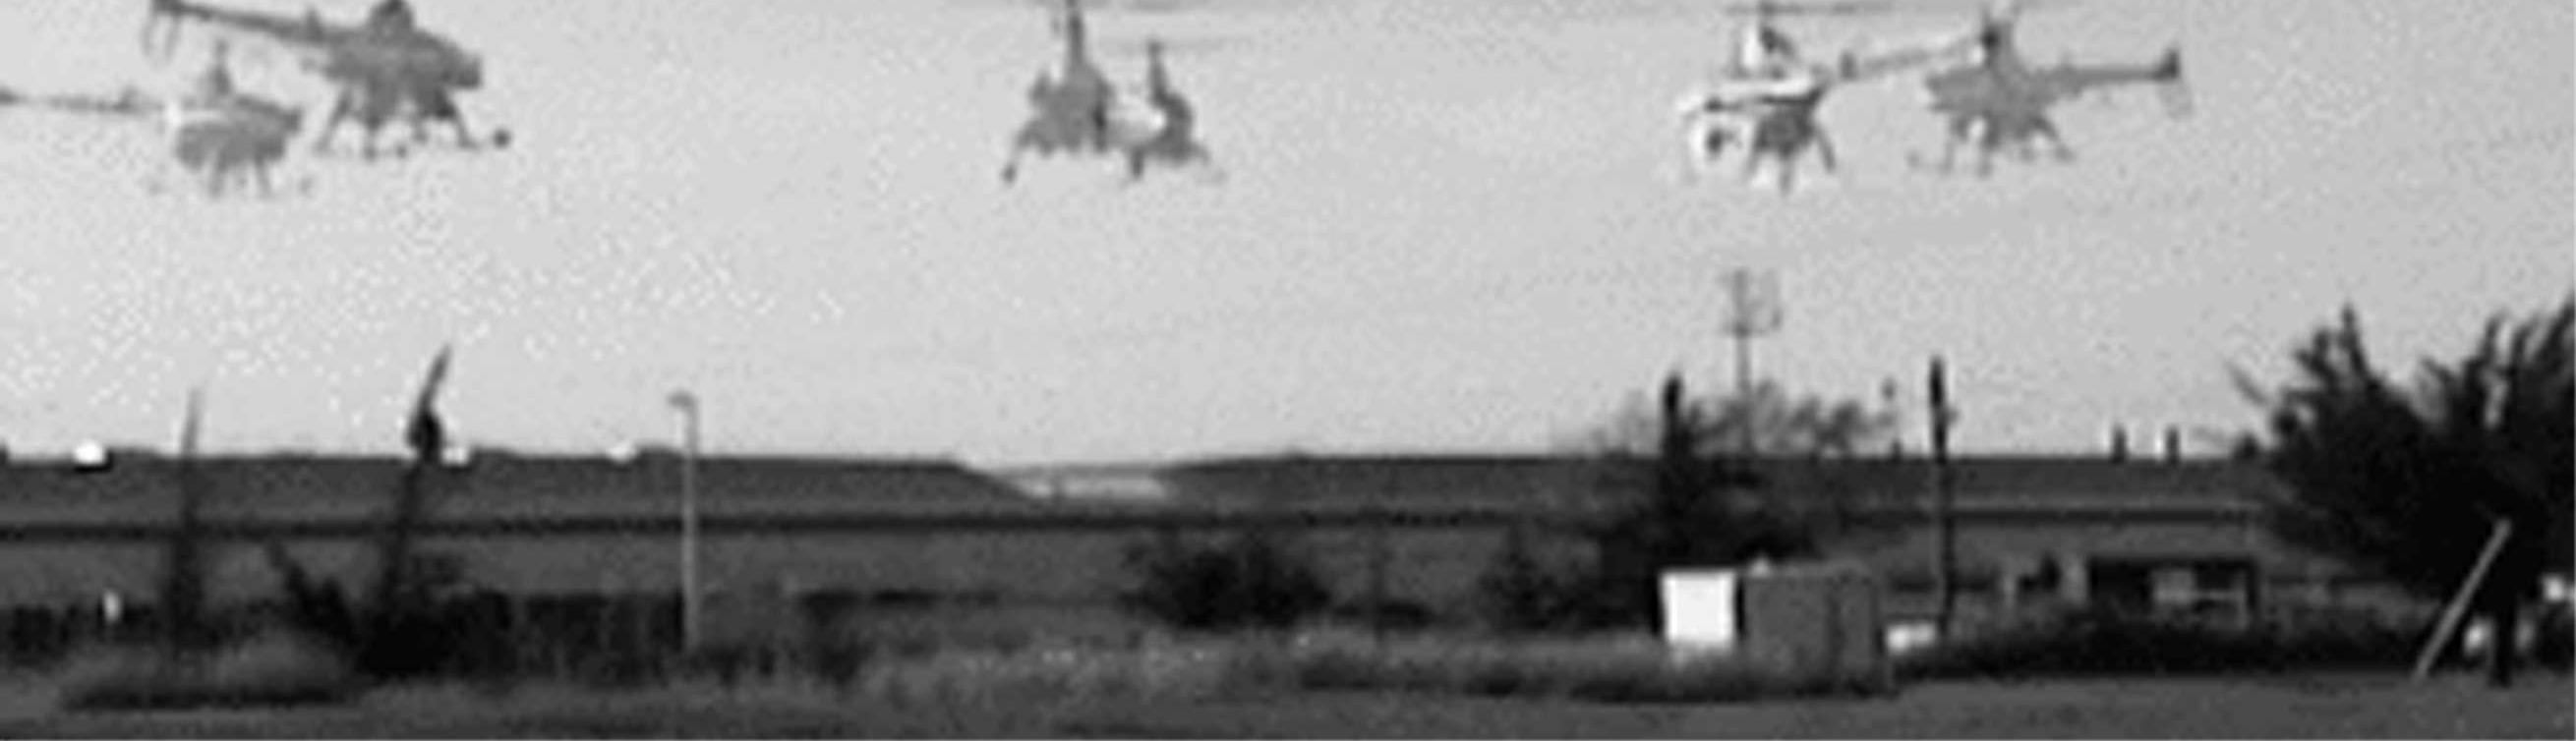
\includegraphics[width=8in]{figures/heliComposite.jpg}}

%%%%%%%%%%%% Slide 8 %%%%%%%%%%%%%%%%%%%%%%%%%%%%%%%%%%%%%%%%%%%%%%%%%%%
\heading{Ví dụ: Trực thăng tự trị}

\vspace*{0.2in}
\centerline{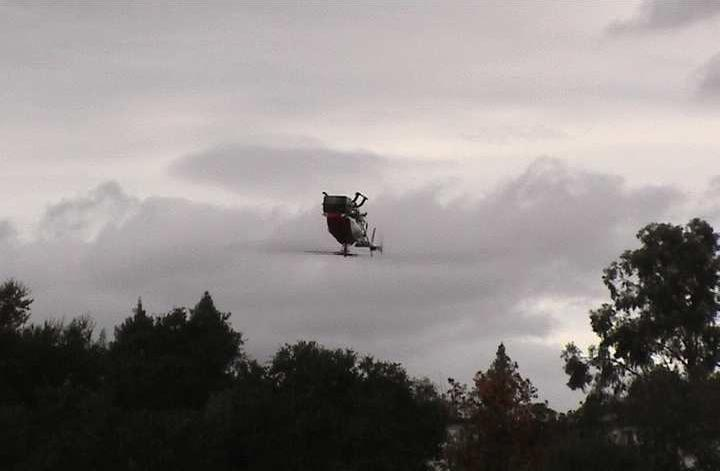
\includegraphics[width=6in]{figures/inverted-hover.jpg}}

%%%%%%%%%%%% Slide 9 %%%%%%%%%%%%%%%%%%%%%%%%%%%%%%%%%%%%%%%%%%%%%%%%%%%
\heading{Học qua khác biệt thời gian (Temporal difference learning)}

\blob Cố định một chính sách $\pi$, thực thi nó, học $U^\pi(s)$

\blob Phương trình Bellman:
\[ U^\pi(s) = R(s) + \gamma \sum_{s'} T(s, \pi(s), s') U^\pi(s') \]

\blob Cập nhật TD điều chỉnh ước tính tiện ích để thống nhất với phương trình Bellman:
\[ U^\pi(s) \leftarrow U^\pi(s) + \alpha \left( R(s) + \gamma U^\pi(s') - U^\pi(s) \right) \]

\blob Về cơ bản sử dụng lấy mẫu từ môi trường thay vì tính tổng chính xác

%%%%%%%%%%%% Slide 10 %%%%%%%%%%%%%%%%%%%%%%%%%%%%%%%%%%%%%%%%%%%%%%%%%%%
\heading{Hiệu suất của TD}

\vspace*{0.2in}
\centerline{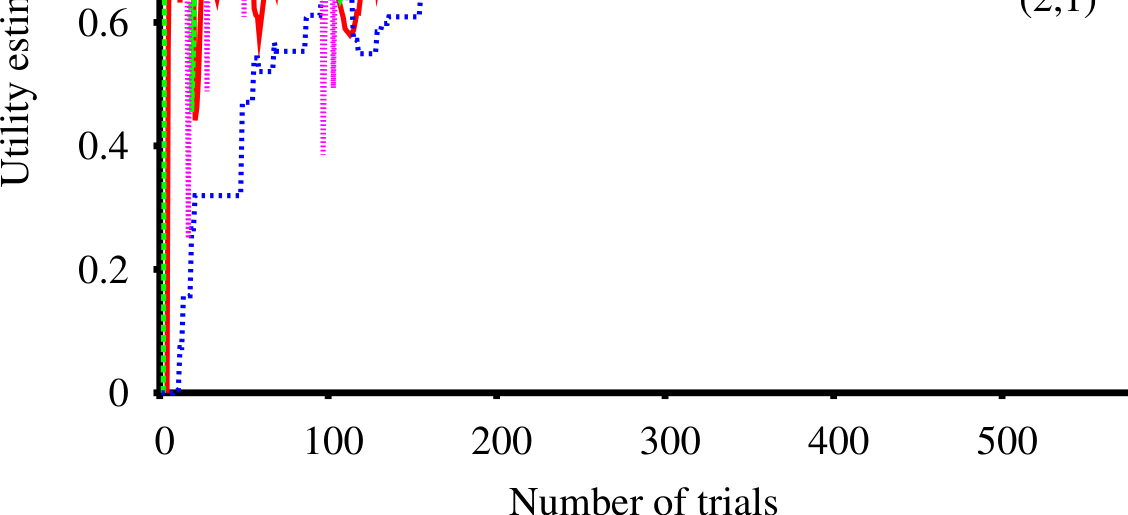
\includegraphics[height=3in]{figures/4x3-passive-td-states.png} \qquad 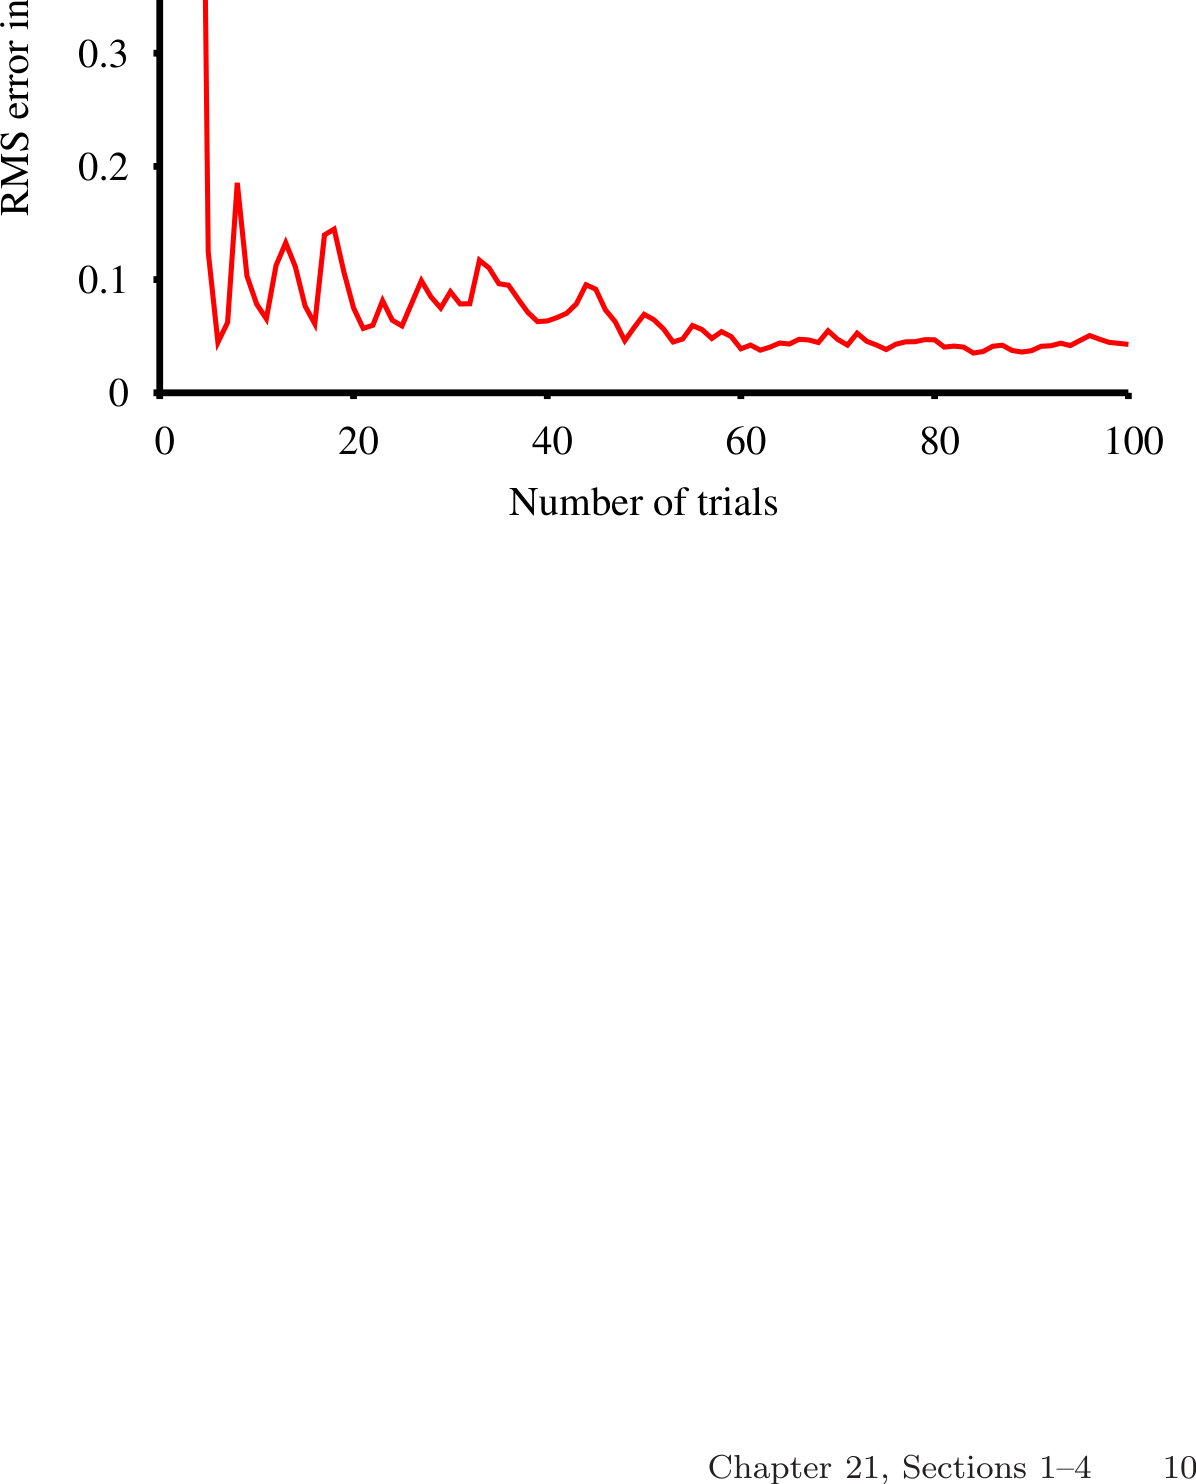
\includegraphics[height=3in]{figures/4x3-passive-td-error.png}}

%%%%%%%%%%%% Slide 11 %%%%%%%%%%%%%%%%%%%%%%%%%%%%%%%%%%%%%%%%%%%%%%%%%%%
\heading{Học Q (Q-learning)}

\blob Một nhược điểm của việc học $U(s)$: vẫn cần $T(s, a, s')$ để đưa ra quyết định

\blob $Q(a,s)$ = tiện ích kỳ vọng nếu chúng ta thực hiện $a$ trong $s$ và sau đó hành động tối ưu

\blob Phương trình Bellman:
\[ Q(a,s) = R(s) + \gamma \sum_{s'} T(s, \pi(s), s') \max_{a'} Q(a', s') \]

\blob Cập nhật Q-learning:
\[ Q(a,s) \leftarrow Q(a,s) + \alpha \left( R(s) + \gamma \max_{a'} Q(a', s') - Q(a,s) \right) \]

\blob Q-learning là một phương pháp không cần mô hình (model-free) để học và ra quyết định
(vì vậy không thể sử dụng mô hình để ràng buộc các giá trị Q, mô phỏng trong tư duy, v.v.)

%%%%%%%%%%%% Slide 12 %%%%%%%%%%%%%%%%%%%%%%%%%%%%%%%%%%%%%%%%%%%%%%%%%%%
\heading{Xấp xỉ hàm (Function approximation)}

\blob Đối với các bài toán thực tế, không thể biểu diễn $U$ hoặc $Q$ dưới dạng bảng!!

\blob Thông thường sử dụng xấp xỉ hàm tuyến tính:
\[ \hat{U}_\theta(s) = \theta_1 f_1(s) + \theta_2 f_2(s) + \dots + \theta_n f_n(s) \]

\blob Sử dụng một bước gradient để sửa đổi các tham số $\theta$:
\[ \theta_i \leftarrow \theta_i + \alpha \left[ R(s) + \gamma \hat{U}_\theta(s') - \hat{U}_\theta(s) \right] \frac{\partial \hat{U}_\theta(s)}{\partial \theta_i} \]

\[ \theta_i \leftarrow \theta_i + \alpha \left[ R(s) + \gamma \max_{a'} \hat{Q}_\theta(a', s') - \hat{Q}_\theta(a,s) \right] \frac{\partial \hat{Q}_\theta(a,s)}{\partial \theta_i} \]

\blob Thường rất hiệu quả trong thực tế, nhưng không đảm bảo sự hội tụ

%%%%%%%%%%%% Slide 13 %%%%%%%%%%%%%%%%%%%%%%%%%%%%%%%%%%%%%%%%%%%%%%%%%%%
\heading{Khám phá (Exploration)}

\blob Tác tử nên cư xử như thế nào? Chọn hành động với tiện ích kỳ vọng cao nhất?

\vspace*{0.2in}
\centerline{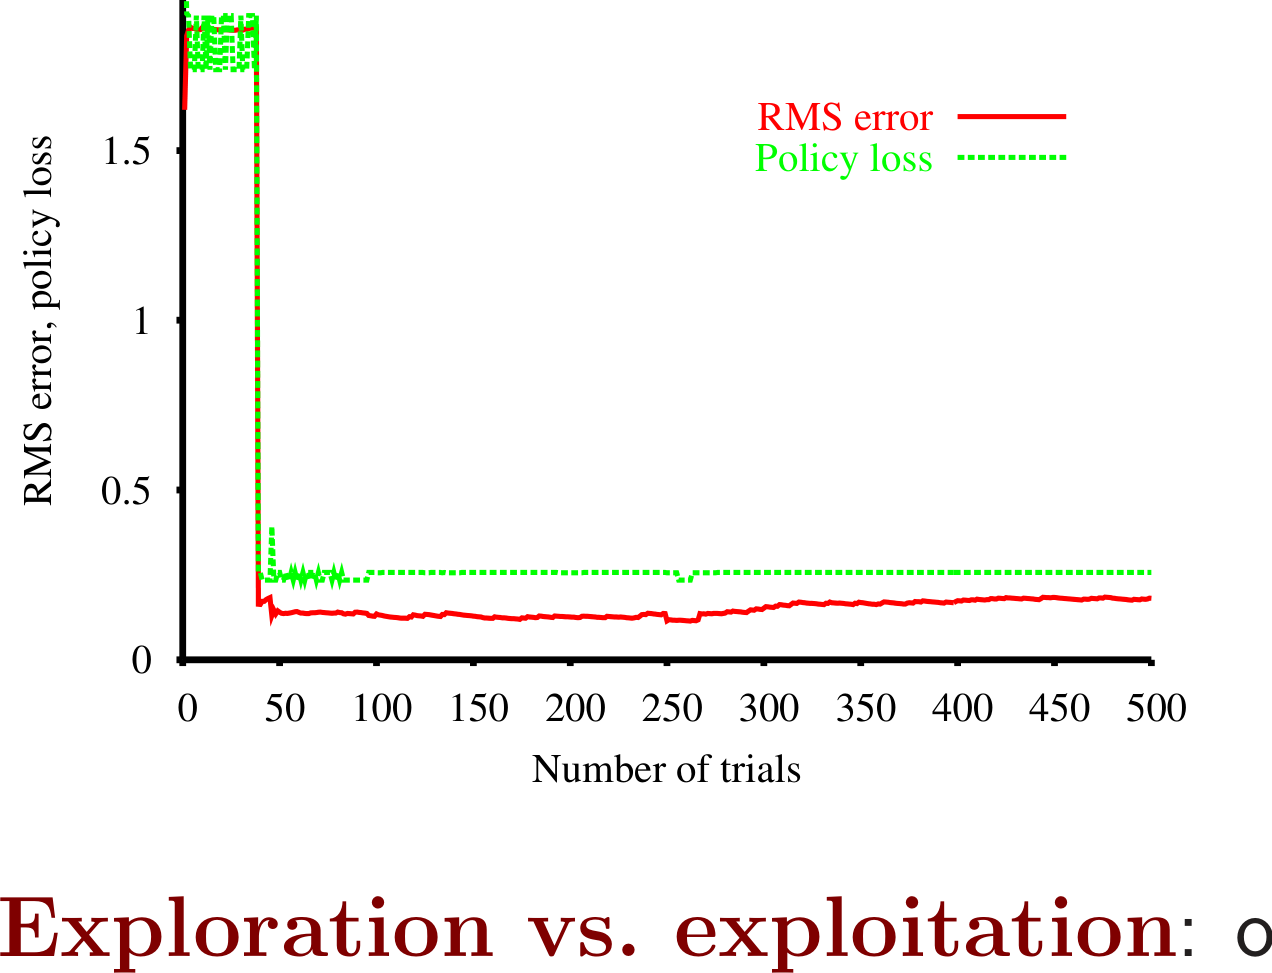
\includegraphics[height=3in]{figures/loss.png} \qquad 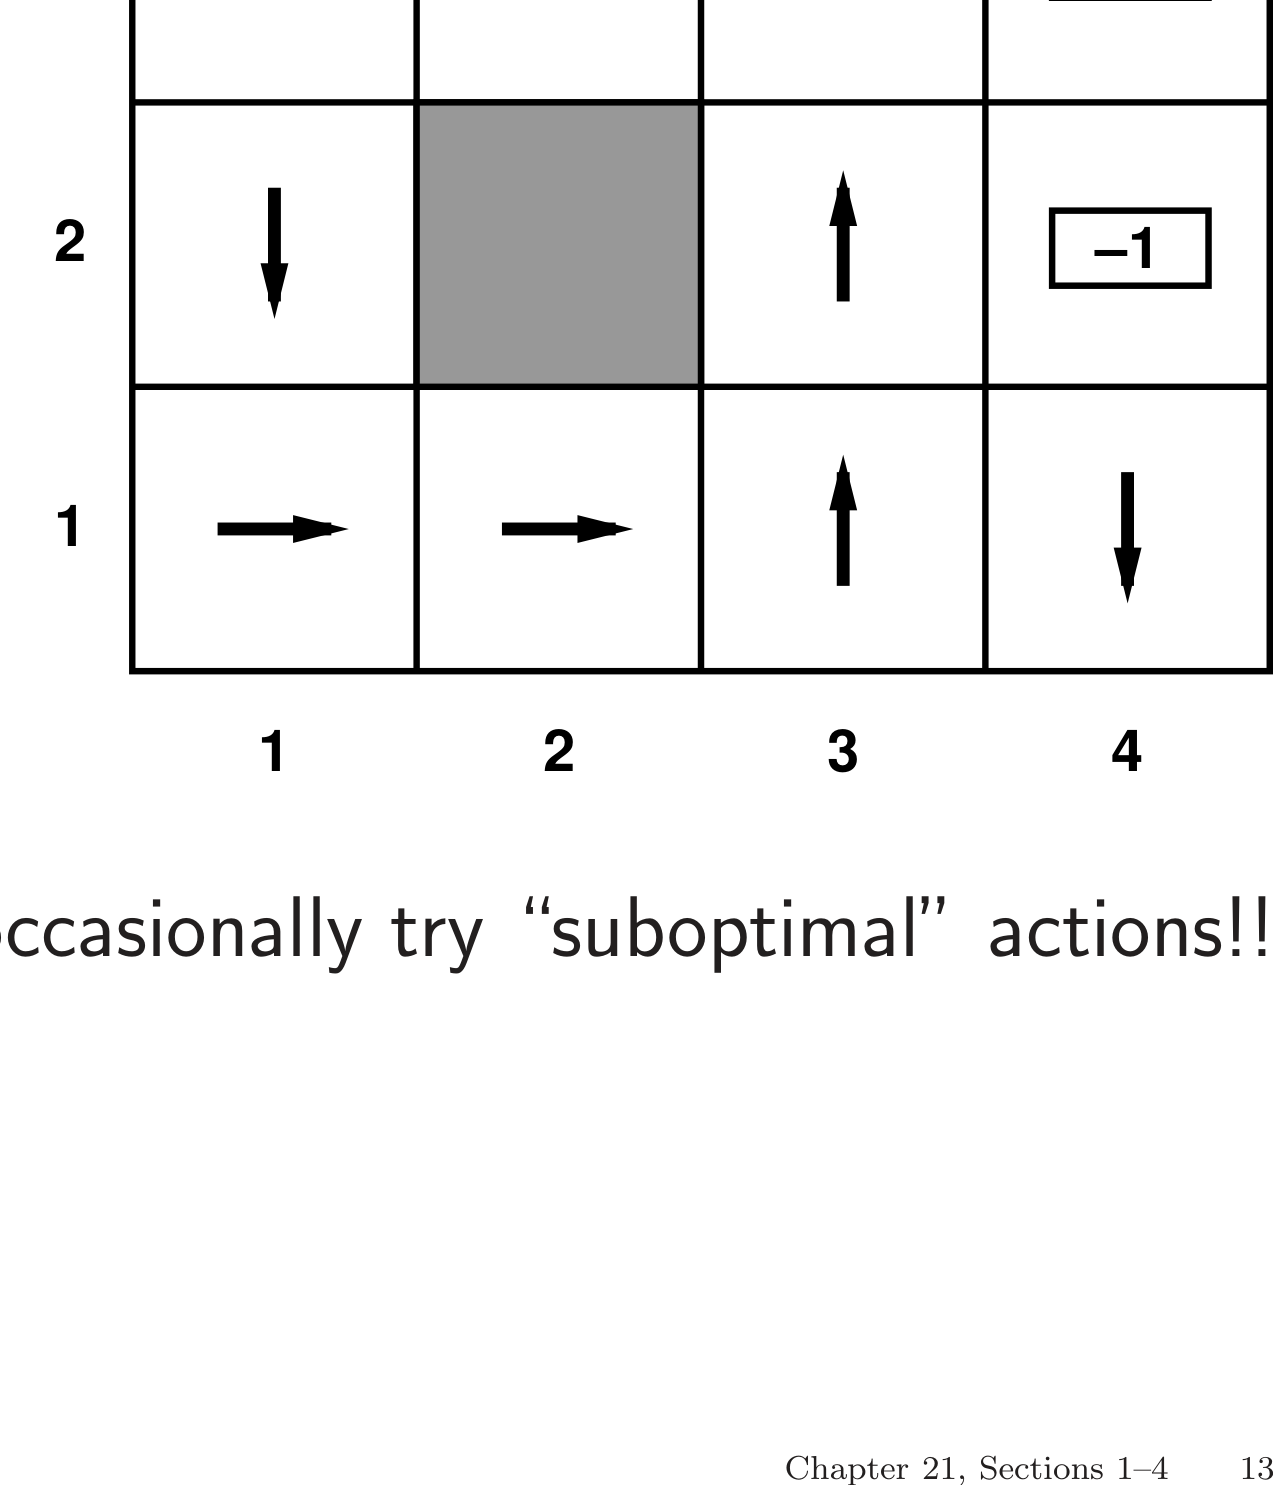
\includegraphics[height=3in]{figures/4x3-greedy-adp-policy.png}}

\blob Khám phá vs. Khai thác (Exploration vs. exploitation): thỉnh thoảng thử các hành động ``dưới mức tối ưu''!!

%%%%%%%%%%%% Slide 14 %%%%%%%%%%%%%%%%%%%%%%%%%%%%%%%%%%%%%%%%%%%%%%%%%%%
\heading{Tóm tắt}

\blob Các phương pháp học tăng cường tìm ra các giải pháp xấp xỉ cho MDP

\blob Làm việc trực tiếp từ kinh nghiệm trong môi trường

\blob Không cần phải được cung cấp mô hình chuyển tiếp từ trước

\blob Q-learning hoàn toàn không cần mô hình (model-free)

\blob Xấp xỉ hàm (ví dụ: kết hợp tuyến tính của các đặc trưng) giúp RL mở rộng cho các MDP rất lớn

\blob Sự khám phá là cần thiết để hội tụ đến các giải pháp tối ưu

\end{huge}
\end{document}
